\documentclass[landscape,twocolumn]{article}
\usepackage[utf8]{inputenc}
\usepackage[margin=2.5cm]{geometry}
\usepackage{amsmath}
\usepackage{amsthm}
\usepackage{amssymb}
\usepackage{mathtools}
\usepackage{pgfplots}
\pgfplotsset{compat=1.18}
\usepackage{graphicx}
\usepackage{enumitem}

% Aumentar el espacio entre columnas
\setlength{\columnsep}{6em} % Puedes ajustar el valor según necesites

% Definiciones para entornos matemáticos
\newtheorem{theorem}{Teorema}[section]
\newtheorem{proposition}[theorem]{Proposición}
\newtheorem{lemma}[theorem]{Lema}
\newtheorem{corollary}[theorem]{Corolario}
\newtheorem{definition}[theorem]{Definición}
\newtheorem{example}{Ejemplo}[section]
\newtheorem{remark}{Observación}[section]
\newtheorem{note}{Nota}[section]

\begin{document}

\section{Distribuciones discretas}
%quiero incluir todas las distribuciones discretas comunmente usadas en probabilidad y estadistica con sus c
% casos de uso, su función de densidad, su función de distribución acumulada, esperanza, media, varianza.

\subsection{Distribución uniforme discreta}
\begin{definition}
Una variable aleatoria $X$ tiene distribución uniforme discreta sobre el conjunto $\{a, a+1, ..., b\}$ si toma cada valor con la misma probabilidad.
\end{definition}

\begin{itemize}
    \item \textbf{Función de masa de probabilidad:}
    \[ P(X = k) = \frac{1}{b-a+1}, \quad k = a, a+1, ..., b \]
    
    \item \textbf{Función de distribución acumulada:}
    \[ F(x) = \begin{cases}
        0 & \text{si } x < a \\
        \frac{\lfloor x \rfloor - a + 1}{b-a+1} & \text{si } a \leq x < b \\
        1 & \text{si } x \geq b
    \end{cases} \]
    
    \item \textbf{Esperanza:} $E(X) = \frac{a+b}{2}$
    
    \item \textbf{Varianza:} $Var(X) = \frac{(b-a+1)^2-1}{12}$
\end{itemize}

\begin{example}
Lanzamiento de un dado justo de 6 caras: $X \sim U(1,6)$
\end{example}

% Gráfica de ejemplo
\begin{center}
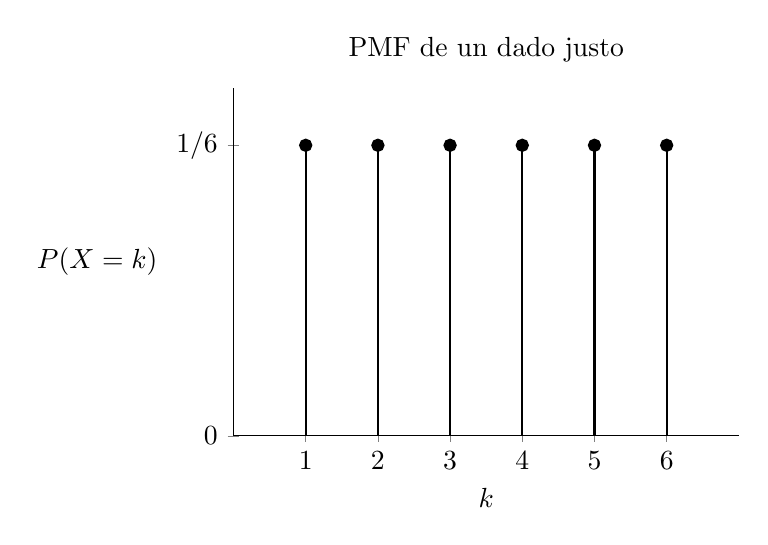
\begin{tikzpicture}
\begin{axis}[
    width=8cm,
    height=6cm,
    xlabel={$k$},
    ylabel={$P(X=k)$},
    ylabel style={rotate=-90},
    ymin=0,
    ymax=0.2,
    xmin=0,
    xmax=7,
    xtick={1,2,3,4,5,6},
    ytick={0,0.167},
    yticklabels={0,1/6},
    title={PMF de un dado justo},
    axis lines=left,  % Solo muestra los ejes x e y
    clip=false,
    axis line style={-},
    every axis plot/.append style={thick}
]
\addplot[ycomb,thick,mark=*] coordinates {
    (1,0.167) (2,0.167) (3,0.167) (4,0.167) (5,0.167) (6,0.167)
};
\end{axis}
\end{tikzpicture}
\end{center}

\subsection{Distribución Bernoulli}
\begin{definition}
Una variable aleatoria $X$ tiene distribución Bernoulli con parámetro $p$ si solo toma dos valores posibles: éxito (1) con probabilidad $p$ y fracaso (0) con probabilidad $1-p$.
\end{definition}

\begin{itemize}
    \item \textbf{Función de masa de probabilidad:}
    \[ P(X = k) = \begin{cases}
        p & \text{si } k = 1 \\
        1-p & \text{si } k = 0
    \end{cases} \]
    
    \item \textbf{Función de distribución acumulada:}
    \[ F(x) = \begin{cases}
        0 & \text{si } x < 0 \\
        1-p & \text{si } 0 \leq x < 1 \\
        1 & \text{si } x \geq 1
    \end{cases} \]
    
    \item \textbf{Esperanza:} $E(X) = p$
    
    \item \textbf{Varianza:} $Var(X) = p(1-p)$
\end{itemize}

\begin{example}
Lanzamiento de una moneda justa: $X \sim Ber(0.5)$
\end{example}

% Gráfica de ejemplo
\begin{center}
\begin{tikzpicture}
\begin{axis}[
    width=8cm,
    height=6cm,
    xlabel={$k$},
    ylabel={$P(X=k)$},
    ylabel style={rotate=-90},
    ymin=0,
    ymax=0.9,
    xmin=-0.5,
    xmax=1.5,
    xtick={0,1},
    ytick={0,0.3, 0.7},
    title={PMF de una moneda cargada},
    axis lines=left,
    clip=false,
    axis line style={-},
    every axis plot/.append style={thick}
]
\addplot[ycomb,thick,mark=*] coordinates {
    (0,0.3) (1,0.7)
};
\end{axis}
\end{tikzpicture}
\end{center}

\end{document}